\documentclass[AdvProjMgmt_Sebastien_Deriaz]{subfiles}


\begin{document}
\section{Planning}
Le projet est séparé en deux phases :
\begin{enumerate}
\item Temps partiel (réalisé en parallèle avec les autres cours)
\item Temps plein (après la fin des cours)
\end{enumerate}
Ces deux phases seront représentées par deux barres bleues sur le Gantt (voir page suivante).\\
Les dates clés sont
\begin{enumerate}
\item 22.02.2021 : Début du projet
\item 21.06.2021 : Début du travail à plein temps
\item 27.08.2021 : Rendu du projet
\item 17.09.2021 : Soutenance de projet
\end{enumerate}
Lors du travail à plein temps, il a été prévu de travailler en parallèle sur les objectifs secondaires ainsi que sur le beta-testing. Si nécessaire, le temps alloué aux objectifs secondaires peut être utilisé pour absorber un éventuel retard sur le projet
\begin{center}
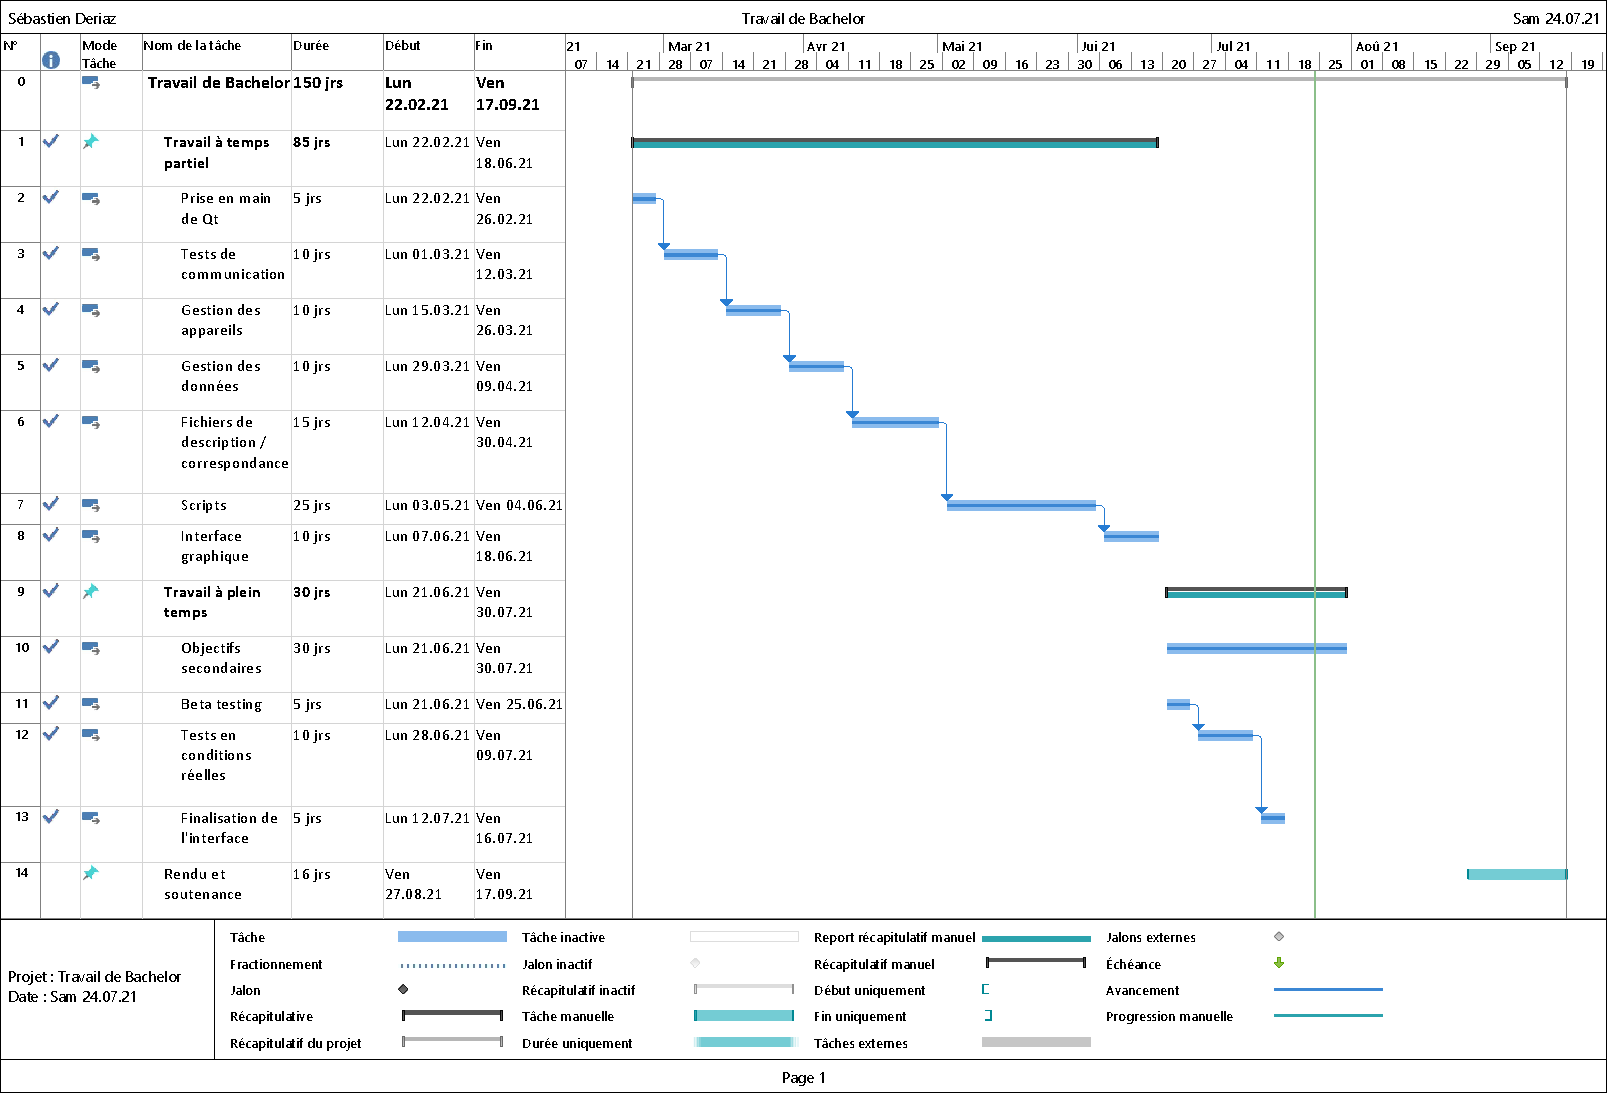
\includegraphics[width=\textheight,angle=90]{Planning_TB.pdf}
\end{center}




\end{document}